\section{Data Security}
\label{sec:sec:data}

The preferred target of an attacker is represented by the data of a person or an organization.
This data can contain critical elements such as passwords, financial data, essential information for the organization's functioning, or plans that should not reach competitors.

In the most common case, the data is read by the attacker and they can use it later directly or indirectly (they can sell it to an interested entity).
Otherwise, an attacker can delete the data or overwrite it.
In this situation, the attacker does not find a utility for the information, but deleting or overwriting it is problematic for the attack victim.

To prevent an attacker's access to data, access permissions must be configured on the respective data, generally stored in files.
In addition to this, to prevent reading the data, especially in case they are transferred through the network, they will be encrypted.
File access permissions and data encryption are the main means of ensuring data confidentiality.

\subsection{Security in the File System}
\label{sec:sec:data:fs}

For correct access to files containing confidential information, modern operating systems allow the configuration of \textbf{access permissions} (\textit{access permissions} or \textit{access rights}).
As we specified above, in the case of these permissions, users and their processes are the subjects, and files are the objects.
In simple form, file permissions are read, write, and execute, as we indicated in \labelindexref{Section}{sec:user:fs-access}.

Thus, an unprivileged user will have write access only in their home directory, will have read access to those system files needed by their processes, and will have no form of access to files with critical system information.
This represents an implementation of the principle of least privilege.
In this implementation, if an attacker gains access to an unprivileged user's account (obtains their password or exploits an application of theirs), they will have limited access to files in the system.

An additional form of protecting access to the file system is using a utility like \cmd{chroot}.
\cmd{chroot} is a Linux utility that changes the root directory of the file system for a process.
Thus, a process will no longer have \file{/} (\textit{slash}) as the root directory, but a subdirectory of it, for example \file{/var/lib/app/}.
In this situation, the process running through \cmd{chroot} will have access only to files in the \file{/var/lib/app/} hierarchy, not to all files in the file system, limiting the damages that would be produced if it were exploited.
This technique is also called \textbf{jailing}.

\subsection{Data Confidentiality}
\label{sec:sec:data:confidentiality}

Modern systems and devices have almost permanent connection to the Internet and transfer information between them.
In this situation, file permissions in the local system are irrelevant for an attacker who can capture the data when it is transferred.
That is why we need ways to hide this data so that, even if captured, it cannot be read by an attacker, that is, to maintain \textbf{data confidentiality}.
Data confidentiality is generally ensured through \textbf{encryption}.

In addition, even on a local system, it is recommended that critical data be encrypted.
If access permissions are not configured appropriately or if an attacker manages to bypass permissions or exploit a privileged process that has access to data, then they will be able to read the critical data.
Encrypting critical data on the local system, beyond appropriately configured access permissions, is a form of \textbf{defense in depth}.

Data encryption assumes that input data is subjected to a process (of encryption) from which hidden output data results.
In cryptology, data is also called \textbf{messages}.
We have, therefore, an input message and an output message.
The input message is called \textbf{intelligible message} (\textit{plaintext}), and the output message is called \textbf{hidden message} (\textit{ciphertext}).
For encrypting a plaintext message into a ciphertext message, an \textbf{encryption algorithm} is needed.
The encryption algorithm is the set of steps through which the plaintext message is processed into the ciphertext message.
The encryption algorithm typically uses an \textbf{encryption key}.
This modifies the algorithm's functioning so that, in the case of the same plaintext message and the same encryption algorithm, but different encryption keys, different ciphertext messages will result.
The functioning of encryption with the four components (plaintext message, ciphertext message, algorithm, and key) is described schematically in \labelindexref{Figure}{fig:sec:encryption}.

\begin{figure}[htbp]
  \centering
  \def\svgwidth{\columnwidth}
  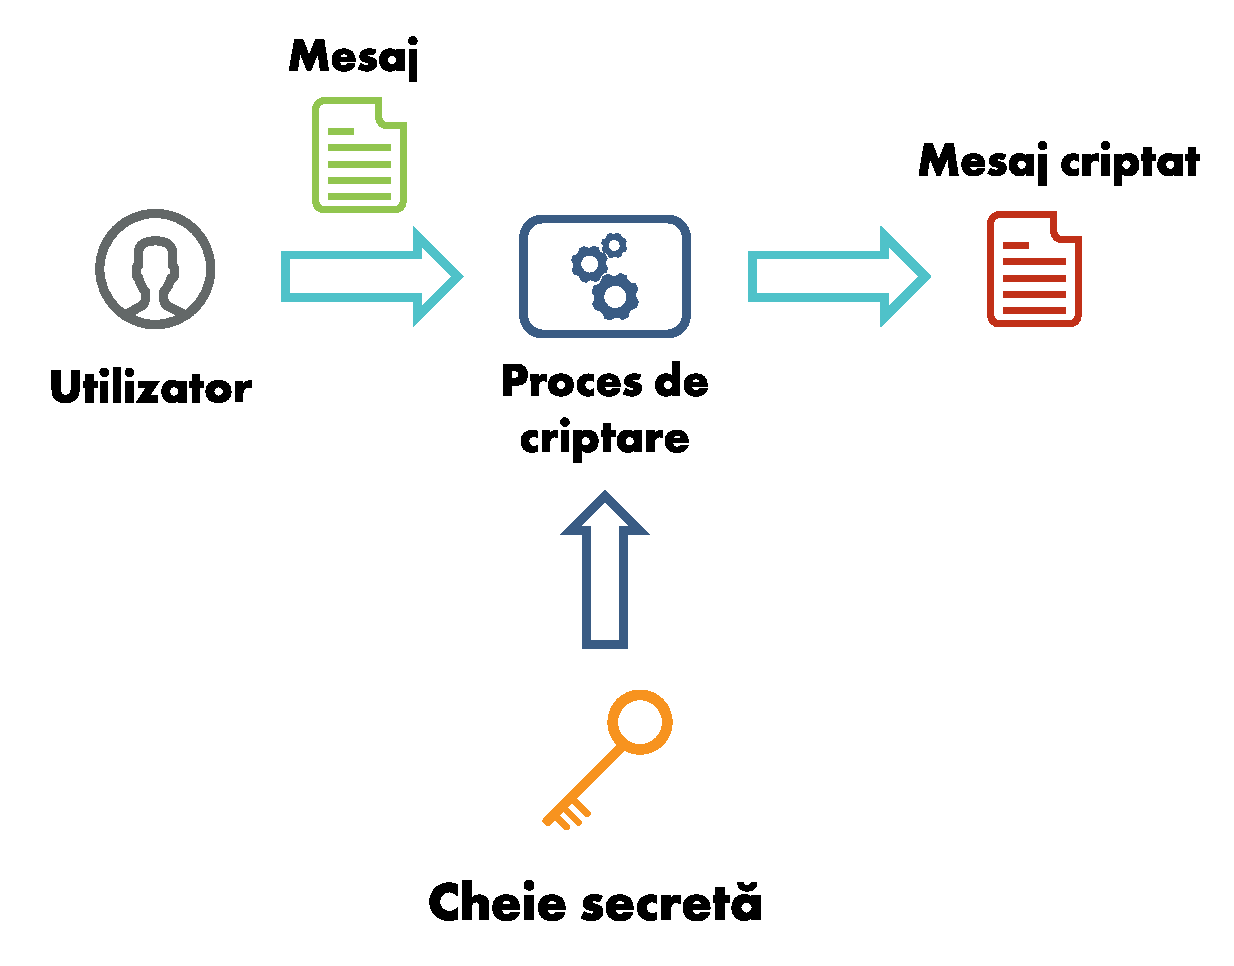
\includegraphics[width=0.6\textwidth]{chapters/12-auth/img/encryption.svg.pdf}
  \caption{Data Encryption}
  \label{fig:sec:encryption}
\end{figure}

A ciphertext message will be hidden from the attacker because they do not know the encryption key.
But it will need to be decrypted by a valid user.
\textbf{Decryption} is the inverse operation of encryption in which the input message is the ciphertext message and the output message is the plaintext message.
To be able to decrypt a ciphertext file, a user needs access to a decryption key and to know the decryption algorithm.
If this key is the same as the encryption key, we say we use symmetric encryption, otherwise we say we use asymmetric encryption.

In the case of \textbf{symmetric encryption}, the same key is used for both encryption and decryption as in \labelindexref{Figure}{fig:sec:symmetric-encryption}.
The most used symmetric encryption algorithm is AES \abbrev{AES}{Advanced Encryption Standard} (\textit{Advanced Encryption Standard}).
The encryption key must be known both by the entity that does the encryption and by the entity that does the decryption.
In the likely case that these entities are in different places on the Internet, the key must be transferred through the network.
For this, key exchange algorithms (\textit{key exchange}) are usually used.
For example, such an algorithm is Diffie-Hellman-Merkle.

\begin{figure}[htbp]
  \centering
  \def\svgwidth{\columnwidth}
  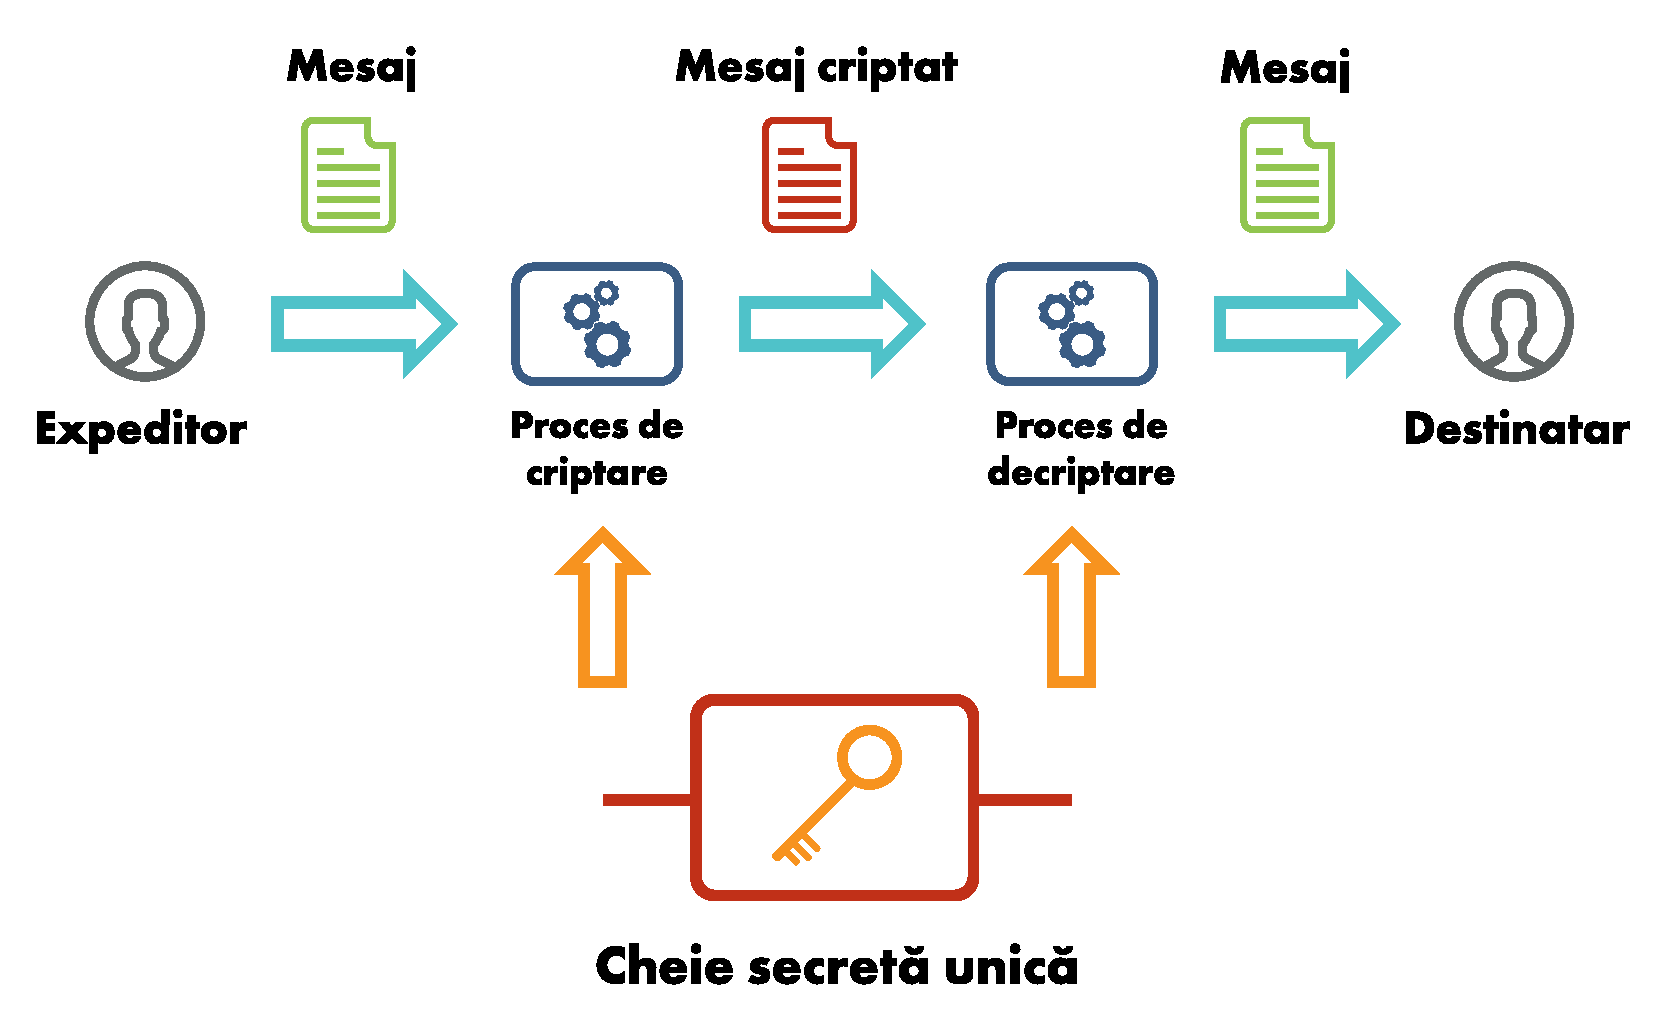
\includegraphics[width=0.7\textwidth]{chapters/12-auth/img/symmetric-encryption.svg.pdf}
  \caption{Symmetric Encryption}
  \label{fig:sec:symmetric-encryption}
\end{figure}

In the case of \textbf{asymmetric encryption}, also called \textbf{public key cryptography} (\textit{public key cryptography}), one key is used for encryption and another for decryption.
The two keys (called private/secret key and public key) are mathematically related.
In general, the private key is generated randomly, and the public key is generated from the private key.
The public key is accessible to the entire world, while the private key is accessible only to the entity that owns it.
Encryption is performed using the public key, and decryption is performed using the private key, as in \labelindexref{Figure}{fig:sec:asymmetric-encryption}.
That is, anyone can encrypt and transmit a message using the public key, but only the holder of the private key can decrypt that message.
The most widespread asymmetric encryption algorithm is RSA\abbrev{RSA}{Rivest-Shamir-Adleman}.
The name comes from its creators (Rivest–Shamir–Adleman).

\begin{figure}[htbp]
  \centering
  \def\svgwidth{\columnwidth}
  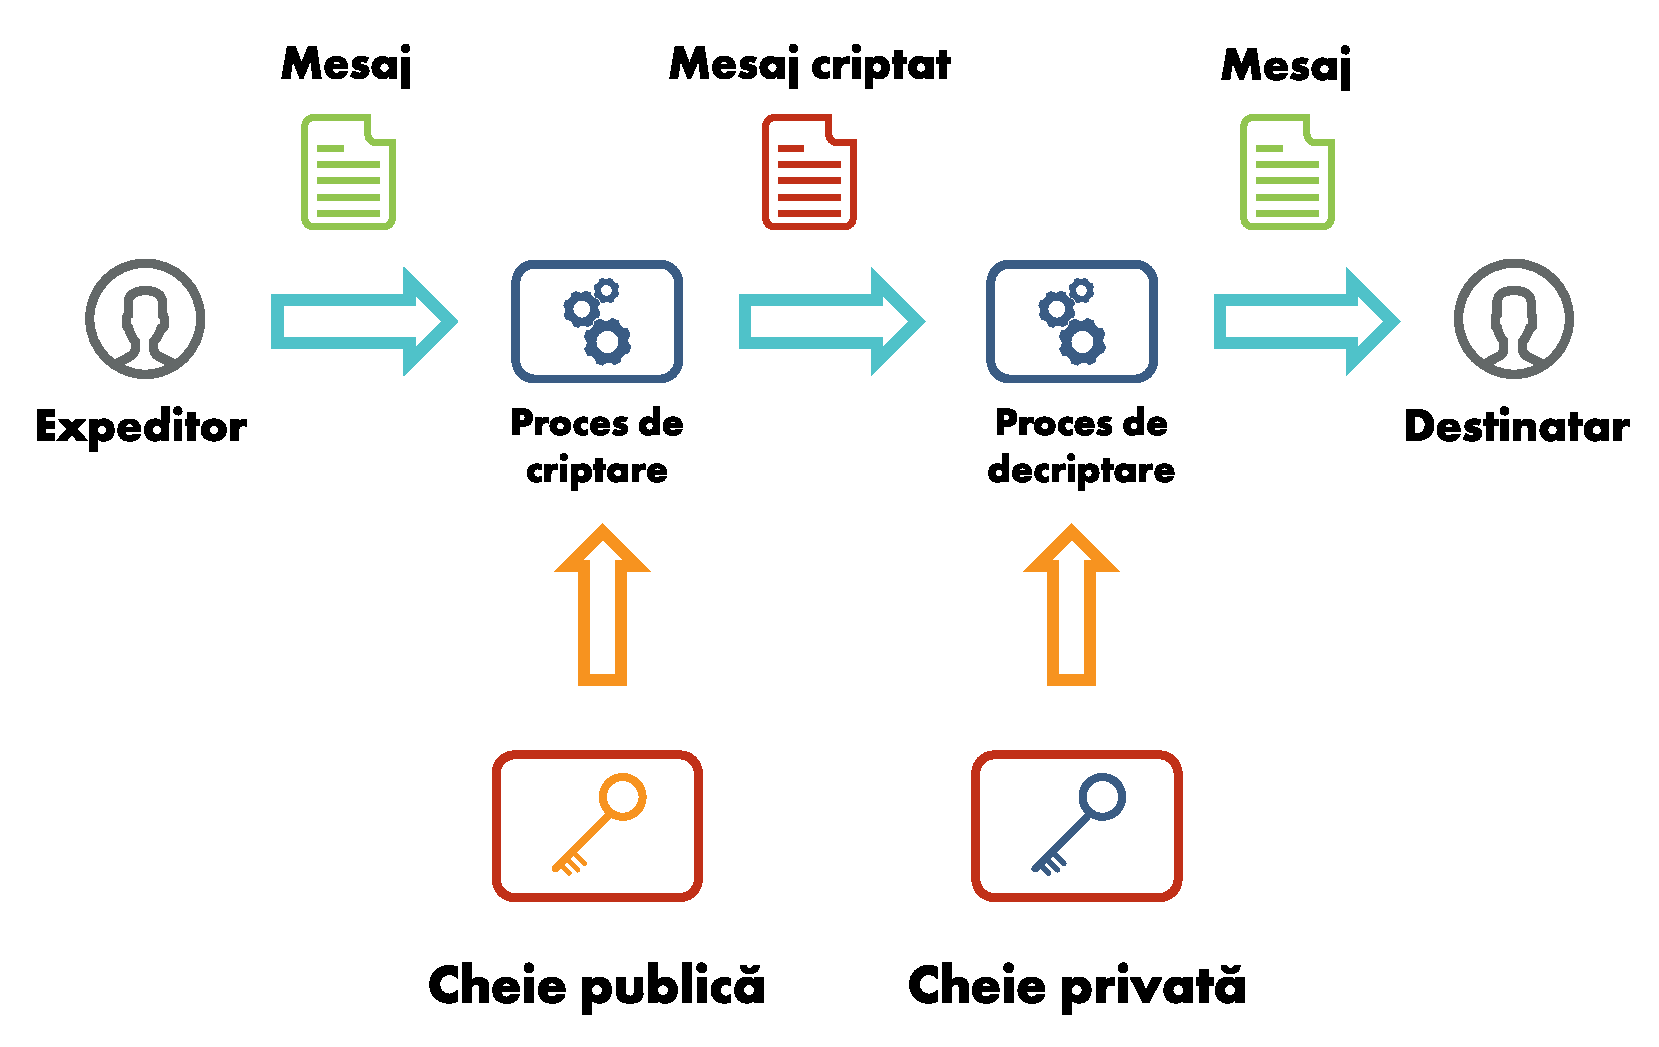
\includegraphics[width=0.7\textwidth]{chapters/12-auth/img/asymmetric-encryption.svg.pdf}
  \caption{Asymmetric Encryption (with public keys)}
  \label{fig:sec:asymmetric-encryption}
\end{figure}

Asymmetric encryption is advantageous because there is no need to transmit a key.
The private key is generated locally and kept locally, and the public key is provided to the general public to use it for transmitting encrypted messages.
In this way, we avoid the drawback of key sharing from symmetric encryption.
The disadvantage of asymmetric encryption is speed: it is less performant than symmetric encryption.
That is why, in practice, asymmetric encryption is used for establishing a secure communication channel based on which the symmetric key is established (only for that session), and then symmetric encryption is used.
This is the operating mode of the Diffie-Hellman-Merkle algorithm.
Succinctly, the algorithm follows the steps below.
We consider two entities (a transmitter and a receiver) and a public communication channel (accessible to the attacker):

\begin{enumerate}
  \item Both entities agree on a shared number (transmitted on the public channel).
  \item Each entity has a private number and generates a private key from the public number and the private number.
    The two keys, although private, have a mathematical relationship given by the shared number.
  \item Each entity generates a public key from the private key and is transmitted to the other entity (on the public channel).
  \item Given the mathematical relationship between the two public keys, the two entities can calculate a new, identical number, which will be the key for symmetric encryption, a key that was not transmitted on the public channel.
\end{enumerate}

Even if an attacker cannot obtain the encryption key, encryption algorithms are not unbeatable.
A weak encryption algorithm can be "broken" by an attacker (i.e., the encryption key can be determined) if the attacker has access to enough ciphertext messages (for example, captured from the network).
This action is called \textbf{cryptanalysis}.
A robust encryption algorithm resists cryptographic attacks and does not allow the discovery of the key when the attacker has access to many ciphertext messages.

Encryption can also be used by the attacker in the case of \textbf{ransomware} attacks.
In this type of attack, the victim's data is not useful to the attacker, but the attacker knows that this data is useful to the victim.
Therefore, they encrypt it and demand a sum of money for the victim to be able to recover the data.
Obviously, the attacker must first be able to reach the data.
So protecting data through access permissions is important.
Another solution is periodic backup of data (which we discussed in \labelindexref{Section}{sec:storage:backup}), which also solves problems of erroneous data deletion or hardware defects of storage devices.

Usually, a user will not directly use encryption utilities.
Encryption algorithms are, in general, implemented in the form of libraries which are then used by applications that use the encryption functionality.
For example, a web browser can use an encryption library to encrypt user-saved passwords in a local file, or a user can decide to encrypt a partition on disk, with the formatting and mounting utilities being responsible for using an encryption library.

One of the most used encryption libraries, generally present in Linux systems, is OpenSSL.
The OpenSSL library also provides a utility that can be used in the command line for encrypting and decrypting data.
In \labelindexref{Listing}{lst:sec:openssl} we use the \cmd{openssl} utility and the AES algorithm to encrypt the file \file{plain.txt} into the file \file{cipher.dat}, and then we decrypt the file \file{cipher.dat} into the file \file{decrypted.txt}.
Finally, we observe that the file \file{decrypted.txt} and the file \file{plain.txt} are identical.
So both operations (encryption and decryption) were performed successfully.

\begin{screen}[caption={Encryption and decryption using openssl},label={lst:sec:openssl}]
student@uso:~$ cat plain.txt
chow time
student@uso:~$ openssl enc -aes256 -in plain.txt -out cipher.dat
enter aes-256-cbc encryption password:
Verifying - enter aes-256-cbc encryption password:
*** WARNING : deprecated key derivation used.
Using -iter or -pbkdf2 would be better.
student@uso:~$ openssl enc -aes256 -in plain.txt -out cipher.dat -pbkdf2
enter aes-256-cbc encryption password:
Verifying - enter aes-256-cbc encryption password:
student@uso:~$ xxd cipher.dat
00000000: 5361 6c74 6564 5f5f 094d d919 9e8c 7558  Salted__.M....uX
00000010: 711b 9862 4488 ddd2 9332 d5ce 66b2 b91d  q..bD....2..f...
student@uso:~$ openssl enc -aes256 -d -in cipher.dat -out decrypted.txt -pbkdf2
enter aes-256-cbc decryption password:
student@uso:~$ cat decrypted.txt
chow time
\end{screen}

\subsection{Data Integrity}
\label{sec:sec:data:integrity}

An attacker can seek to read the data, or, in case they are encrypted, can decide to modify them.
This will prevent the data receiver from using them or will use them in an inappropriate manner, beneficial to the attacker.
Even in the absence of an attacker, data can be corrupted by hardware defects of storage devices or network devices.
That is why it is necessary that, in case of data transfer, we ensure their integrity.

Data integrity is generally achieved with hashing algorithms.
A hashing algorithm generates a small-sized summary for an input message.
A file no matter how large will have a summary of only a few tens of bytes, called \textbf{checksum} (\textit{checksum}).
Common hashing algorithms are MD5 or SHA.
The receiver of a message will also receive the checksum of this message and will be able to verify that the message is correct by applying the hashing algorithm over the message and comparing the result with the received checksum.
The generation of the checksum and its verification are presented in \labelindexref{Figure}{fig:sec:checksum}.

\begin{figure}[htbp]
  \centering
  \def\svgwidth{\columnwidth}
  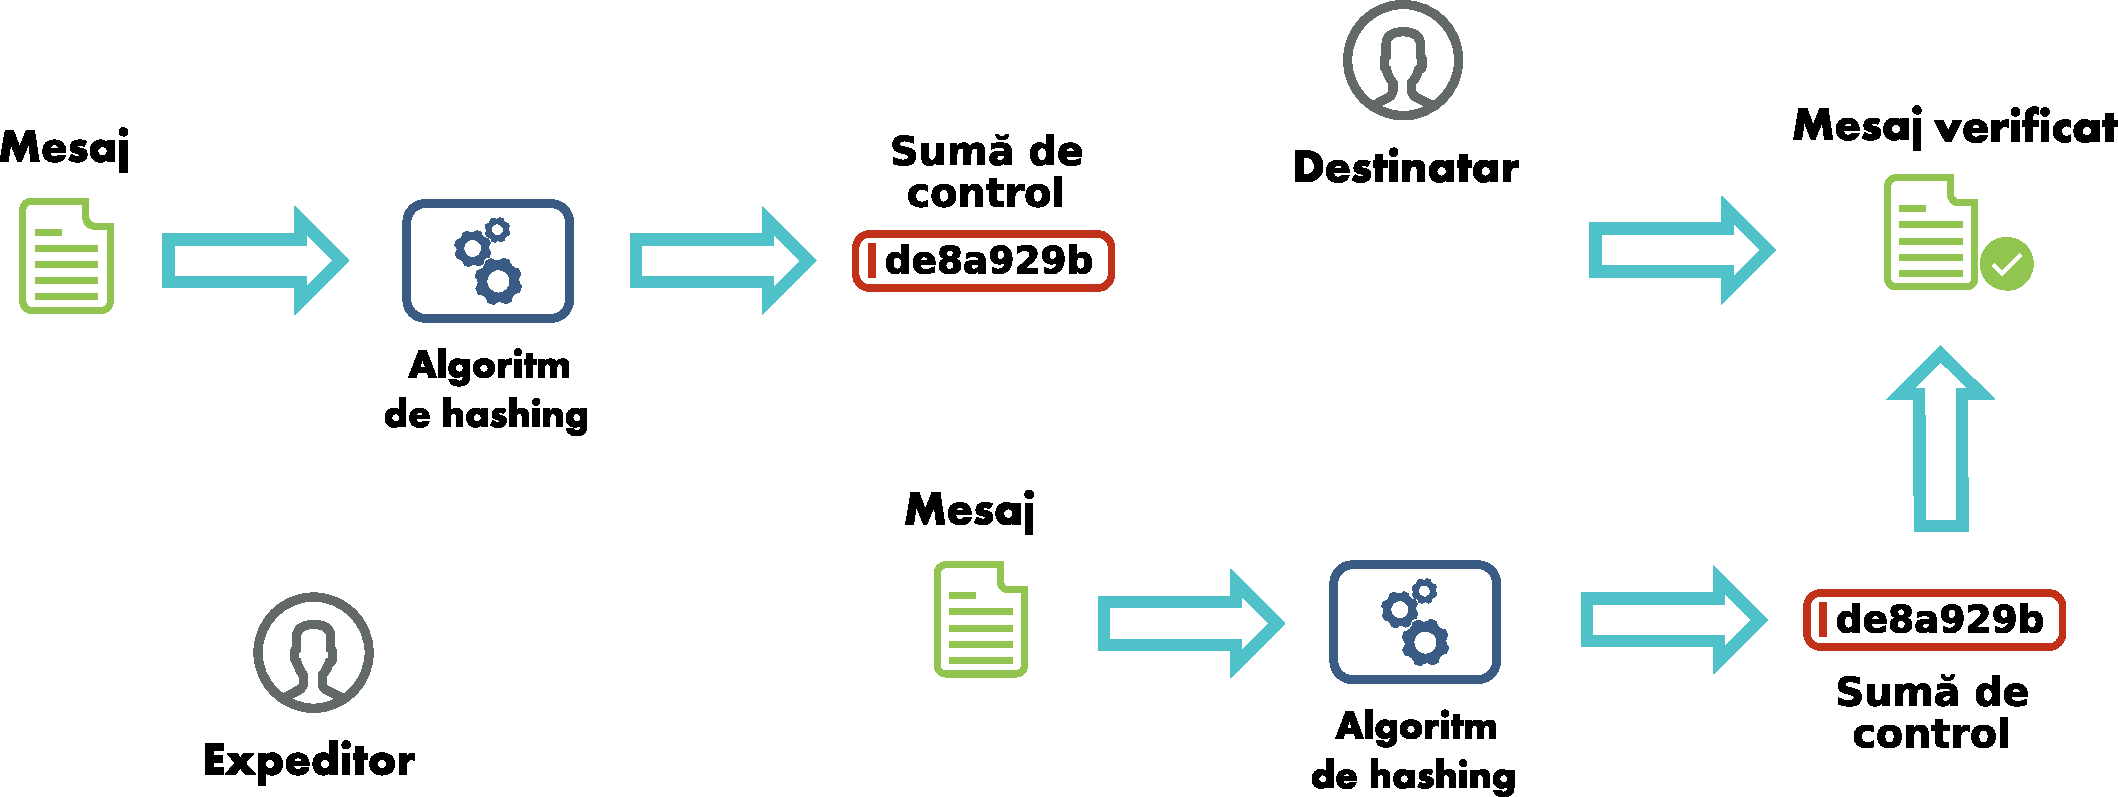
\includegraphics[width=0.9\textwidth]{chapters/12-auth/img/checksum.svg.pdf}
  \caption{Generation and verification of checksum}
  \label{fig:sec:checksum}
\end{figure}

In the case of a hashing algorithm, multiple input messages (of large sizes) can generate the same summary.
We call this situation a \textbf{collision} (\textit{collision}).
For this situation not to be abused, a hashing algorithm must be collision-resistant (\textit{collision resistance}) and it must be quasi-impossible for an attacker to provide a message different from the initial one that generates the same summary.

Just like in the case of encryption algorithms, hashing algorithms are incorporated into libraries like OpenSSL.
Applications that transfer data through the network, such as BitTorrent clients, will use the hashing algorithm implementations from these libraries to guarantee the integrity of transferred data.
In Linux, there are utilities that implement hashing algorithms for working with files.
For example, if we transfer a large file, such as a virtual machine image, it is recommended to also transfer its summary so that those who will download it can ensure that the data is intact.
In \labelindexref{Listing}{lst:sec:checksum} we use the utilities \cmd{md5sum} and \cmd{sha256sum} to calculate the MD5 and SHA-256 summary for a large virtual machine image (\texttt{12GB}).

\begin{screen}[caption={Checksum calculation},label={lst:sec:checksum}]
student@uso:~$ md5sum SSS-Kali-amd64.ova
3dbd973d2a331e5e755e7949274da626  SSS-Kali-amd64.ova
student@uso:~$ sha256sum SSS-Kali-amd64.ova
caefeebfba5bb19c2acb7f77b373653e5a3179ddf46bb68ddbcad612b545debb  SSS-Kali-amd64.ova
student@uso:~$ ls -sh SSS-Kali-amd64.ova
12G SSS-Kali-amd64.ova
\end{screen} 